\documentclass[border={10pt, 10pt, 10pt, 10pt}]{standalone}

\usepackage{tikz}
\usetikzlibrary{arrows}
\usepackage{graphicx}
\usepackage{varwidth}

\renewcommand\familydefault{\sfdefault}

\begin{document}
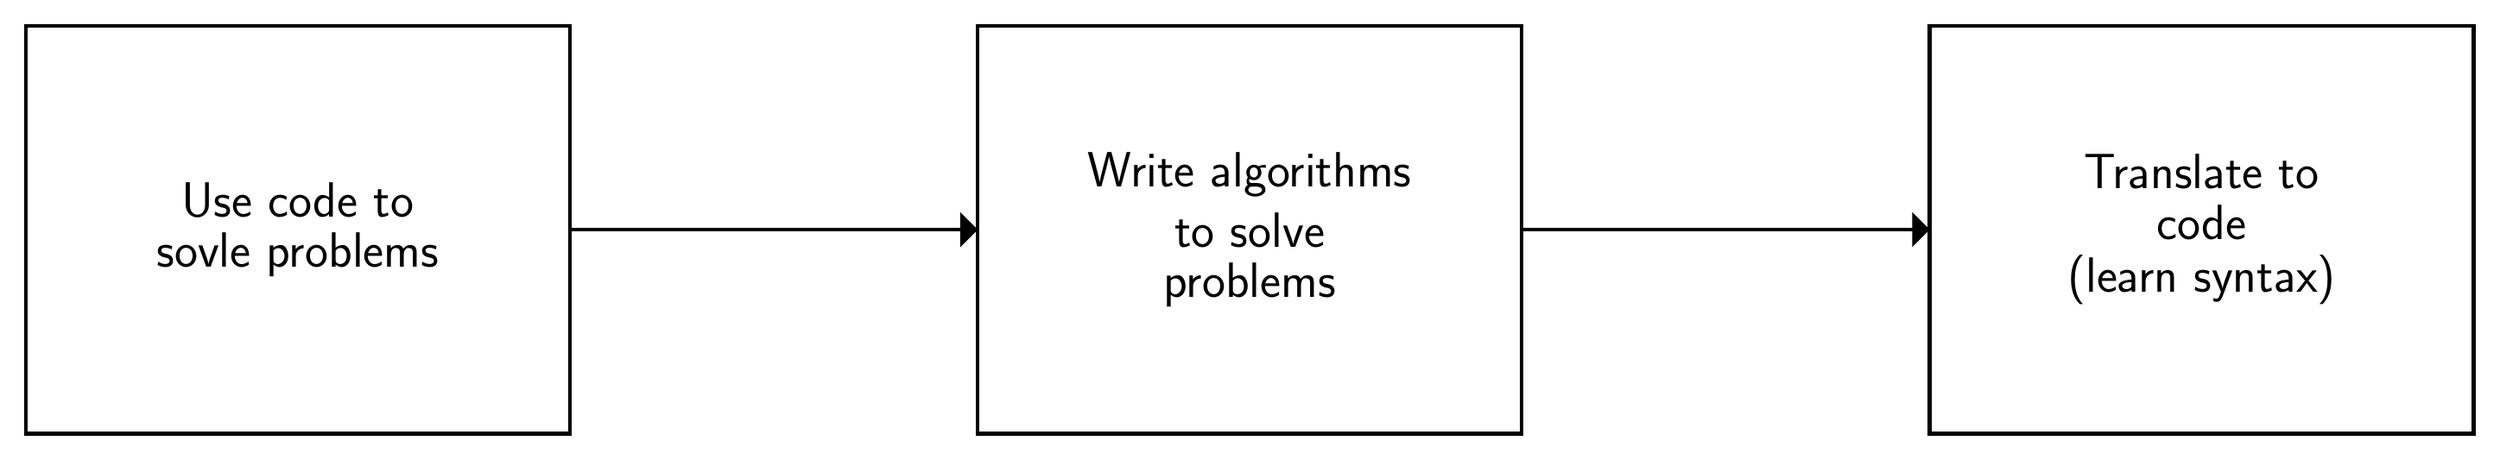
\begin{tikzpicture}

\draw[ultra thick] (-4, -3) rectangle (4, 3);
\draw[ultra thick] (10, -3) rectangle (18, 3);
\draw[ultra thick] (24, -3) rectangle (32, 3);

\node[align=center] at (0, 0) {\huge Use code to\\[2mm]\huge sovle problems};
\node[align=center] at (14, 0) {\huge Write algorithms\\[2mm]\huge to solve\\[2mm]\huge problems};
\node[align=center] at (28, 0) {\huge Translate to\\[2mm]\huge code\\[2mm]\huge (learn syntax)};

\draw[ultra thick, -triangle 90] (4, 0) -- (10, 0);
\draw[ultra thick, -triangle 90] (18, 0) -- (24, 0);

\end{tikzpicture}
\end{document}